\chapter{Redes Neuronales Bayesianas en RISC-V}

En esta sección se explican los pasos y bibliotecas desarrolladas para poder ejecutar inferencia de BNN de manera eficiente en un procesador RISC-V con solo soporte para precisión entera. La Figura \ref{fig:experiment_pipeline} muestra el proceso y componentes necesarios.

\begin{figure}[h]
    \centering
    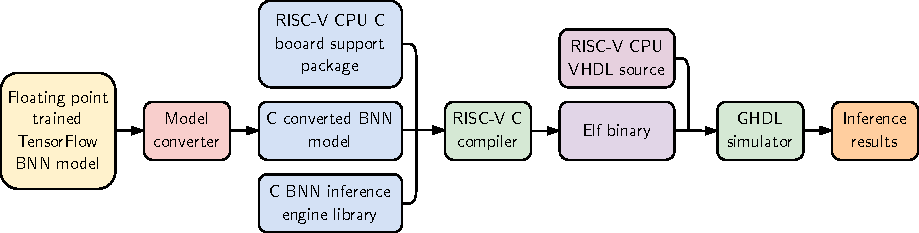
\includegraphics[width=\textwidth]{root/Imagenes/4_bnn_riscv/experiment_pipeline.pdf}
    \caption{\todo}
    \label{fig:experiment_pipeline}
\end{figure}

\section{Componentes desarrollados}

Para poder llevar a cabo el proceso de la Figura \ref{fig:experiment_pipeline} se han realizado las siguientes tareas: actualizar el \textit{\textbf{B}oard \textbf{S}upport \textbf{P}ackage} (BSP) del procesador, desarrollar un motor de inferencia de BNN, desarrollar un conversor de modelos y desarrollar una herramienta de análisis de resultados.

\subsection{Actualización del Board Support Package}

Con el objetivo de mejorar la experiencia de desarrollo del motor de inferencia se actualizó el BSP del procesador para dar soporte a la biblioteca estándar C (libc) y algunas funcionalidades de C++. De esta forma se pueden utilizar funciones útiles de libc cómo \texttt{printf}, o \texttt{memset} entre otras. Para ello se actualizaron las herramientas y ficheros de compilación, se añadieron funciones \textit{stub} para las llamadas al sistema no implementadas y se implementaron versiones modificadas de \texttt{\_write} y \texttt{\_exit}.

\subsection{Motor de inferencia} \label{sec:motor_inferencia_c}

Se ha desarrollado una librería de funciones que ejecutan la inferencia de capas BNN estándar y convolucionales con funciones de activación ReLU o exponenciales normalizadas (SoftMax) utilizando precisión de coma fija. 

\subsubsection{Precisión en coma fija}

Implementar aritmética de coma flotante en hardware es caro, por lo que es común que procesadores de bajas prestaciones no dispongan de dicho hardware. GCC permite emular las operaciones de coma flotante mediante software, comúnmente conocido como \textit{soft-float}. Esta emulación tiene un gran impacto en el rendimiento por lo que no se ha utilizado.

Se ha utilizado el formato coma fija para representar los números decimales en el motor de inferencia. Este formato permite representar números decimales y operar con ellos utilizando hardware de precisión entera, lo que tiene un impacto muy pequeño en el rendimiento. Esta codificación consiste en multiplicar los números con una escala potencia de 2. A mayor sea la escala mayor precisión se obtiene. La principal limitación de esta codificación es el tamaño de palabra de la arquitectura ya que pueden ocurrir desbordamientos al operar con números multiplicados por una escala grande. Por lo que en general se obtiene menor precisión que con la codificación en punto flotante.

\subsubsection{Aproximación de la función SoftMax}

Mientras que calcular la función ReLU es trivial la función SoftMax no. Dicha función toma un vector de componentes $x \in X$ de tamaño $N$ como entrada y devuelve otro del mismo tamaño cuyos componentes $y\in Y$ se calculan según la Ecuación \ref{eq:softmax}.
\begin{equation} \label{eq:softmax}
y_i = \dfrac{e^{x_i}}{\sum_{j = 0}^N e^{x_j}}
\end{equation}

Para calcular esta función utilizando coma fija es necesario calcular la función exponencial en dicho formato. Para evitar desbordamientos de la función exponencial se va a utilizar la función SoftMax equivalente mostrada en la Ecuación \ref{eq:softmax_neg}.
\begin{equation} \label{eq:softmax_neg}
y_i = \dfrac{e^{x_i - \max(X)}}{\sum_{j = 0}^N e^{x_j - \max(X)}}
\end{equation}

En esta versión de la función se cumple que $x_i \in (-\infty, 0]$ por lo que $e^{x_i} \in (0,1]$. Para calcular la función exponencial se va a utilizar la Ecuación \ref{eq:split_exp}, dividiendo la entrada $x_i$ en su parte entera $a_i$ y su parte decimal $b_i$.
\begin{equation} \label{eq:split_exp}
e^{x_i} = e^{a_i+b_i} = e^{a_i} e^{b_i}
\end{equation}

La parte entera $e^{a_i}$ se calcula mediante una LUT de 20 entradas para el rango $[e^{-19}, e^{0}]$. A partir de $e^{-19}$ los valores son demasiado pequeños como para representarlos con la precisión disponible por lo que siempre valen $0$. La parte decimal $e^{b_i}$ se aproxima mediante los 8 primeros términos de la serie de Taylor mostrada en la Ecuación \ref{eq:exp_taylor}. Para optimizar y evitar las divisiones los valores de $\dfrac{1}{n!}$ para $n \in [2,7]$ se han almacenado en una LUT.
\begin{equation} \label{eq:exp_taylor}
e^{b_i} \approx \sum_{n=0}^{7} \dfrac{{b_i}^n}{n!}
\end{equation}

La Figura \ref{fig:exp_aprox} muestra un estudio de la precisión de la aproximación. Se comparan sus resultados con los de la implementación de la función exponencial de la biblioteca estándar en punto flotante. Como medida cuantitativa del error se ha utilizado el error cuadrático medio (\textit{\textbf{M}ean \textbf{S}quared \textbf{E}rror}). Se aprecia como se obtiene una buena aproximación en el rango deseado.

\begin{figure}[h]
    \centering
    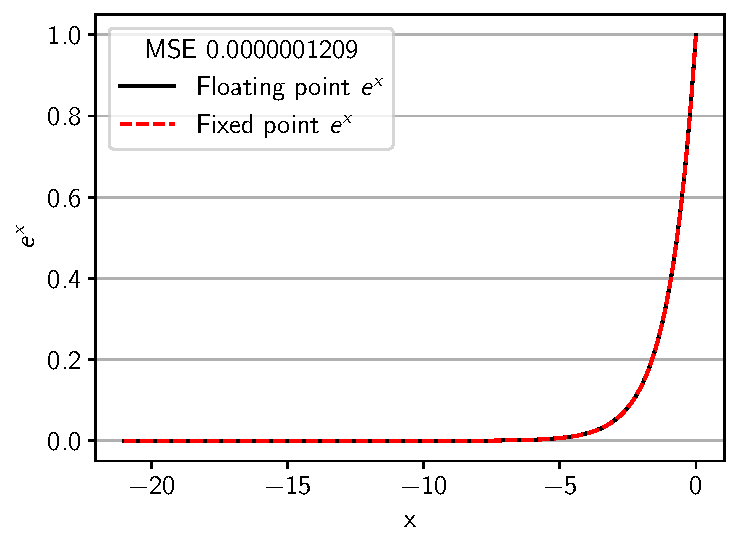
\includegraphics[width=0.55\linewidth]{root/Imagenes/4_bnn_riscv/exp_aprox.pdf}
    \caption{Comparación de la función $e^x$ de la biblioteca estándar en punto flotante (linea negra) con la aproximación en coma fija implementada (linea roja discontinua) en el rango $[-20,0]$.}
    \label{fig:exp_aprox}
\end{figure}

\subsubsection{Aproximación de la función logaritmo}

Para calcular las métricas de incertidumbre se necesita la función logaritmo por lo que se ha implementado una versión del algoritmo desarrollado por Turner \cite{binary_log} para calcular el logaritmo de un número en coma fija.

\subsubsection{Muestreo de la distribución Gaussiana estándar}

Como se ha explicado previamente, las BNN necesitan muestrear distribuciones gaussianas. Como método de muestreo base se utilizada un algoritmo basado en la suma de distribuciones uniformes, dicha suma se aproximan a una distribución gaussiana debido al TCL, como se muestra en la Ecuación \ref{eq:tcl_unif}.
\begin{equation} \label{eq:tcl_unif}
\sum_{n=0}^{N} \mathcal{U}_n(0,1) \sim \mathcal{N} \left( \dfrac{N}{2}, \sqrt{\dfrac{N}{12}} \right)
\end{equation}

El algoritmo implementado genera muestras de $\mathcal{N}(0,1)$ para luego transformarlas en muestras de una distribución gaussiana arbitraria $\mathcal{N}(\mu, \sigma)$ de media $\mu$ y desviación típica $\sigma$ utilizando la Ecuación \ref{eq:gauss_linear}.
\begin{equation} \label{eq:gauss_linear}
\mathcal{N}(\mu, \sigma) = \sigma \mathcal{N}(0,1) + \mu
\end{equation}

Para ello utiliza la suma de 12 distribuciones uniformes y posteriormente centra la distribución como muestra la Ecuación \ref{eq:tcl_12center}.
\begin{equation} \label{eq:tcl_12center}
\sum_{n=0}^{12} \mathcal{U}_n(0,1) - 6 \sim \mathcal{N}(0,1)
\end{equation}

La Figura \ref{fig:gauss_aprox} muestra un análisis estadístico del método de muestreo implementado. En el gráfico Q-Q se aprecia como el histograma 

\begin{figure}[h]
    \centering
    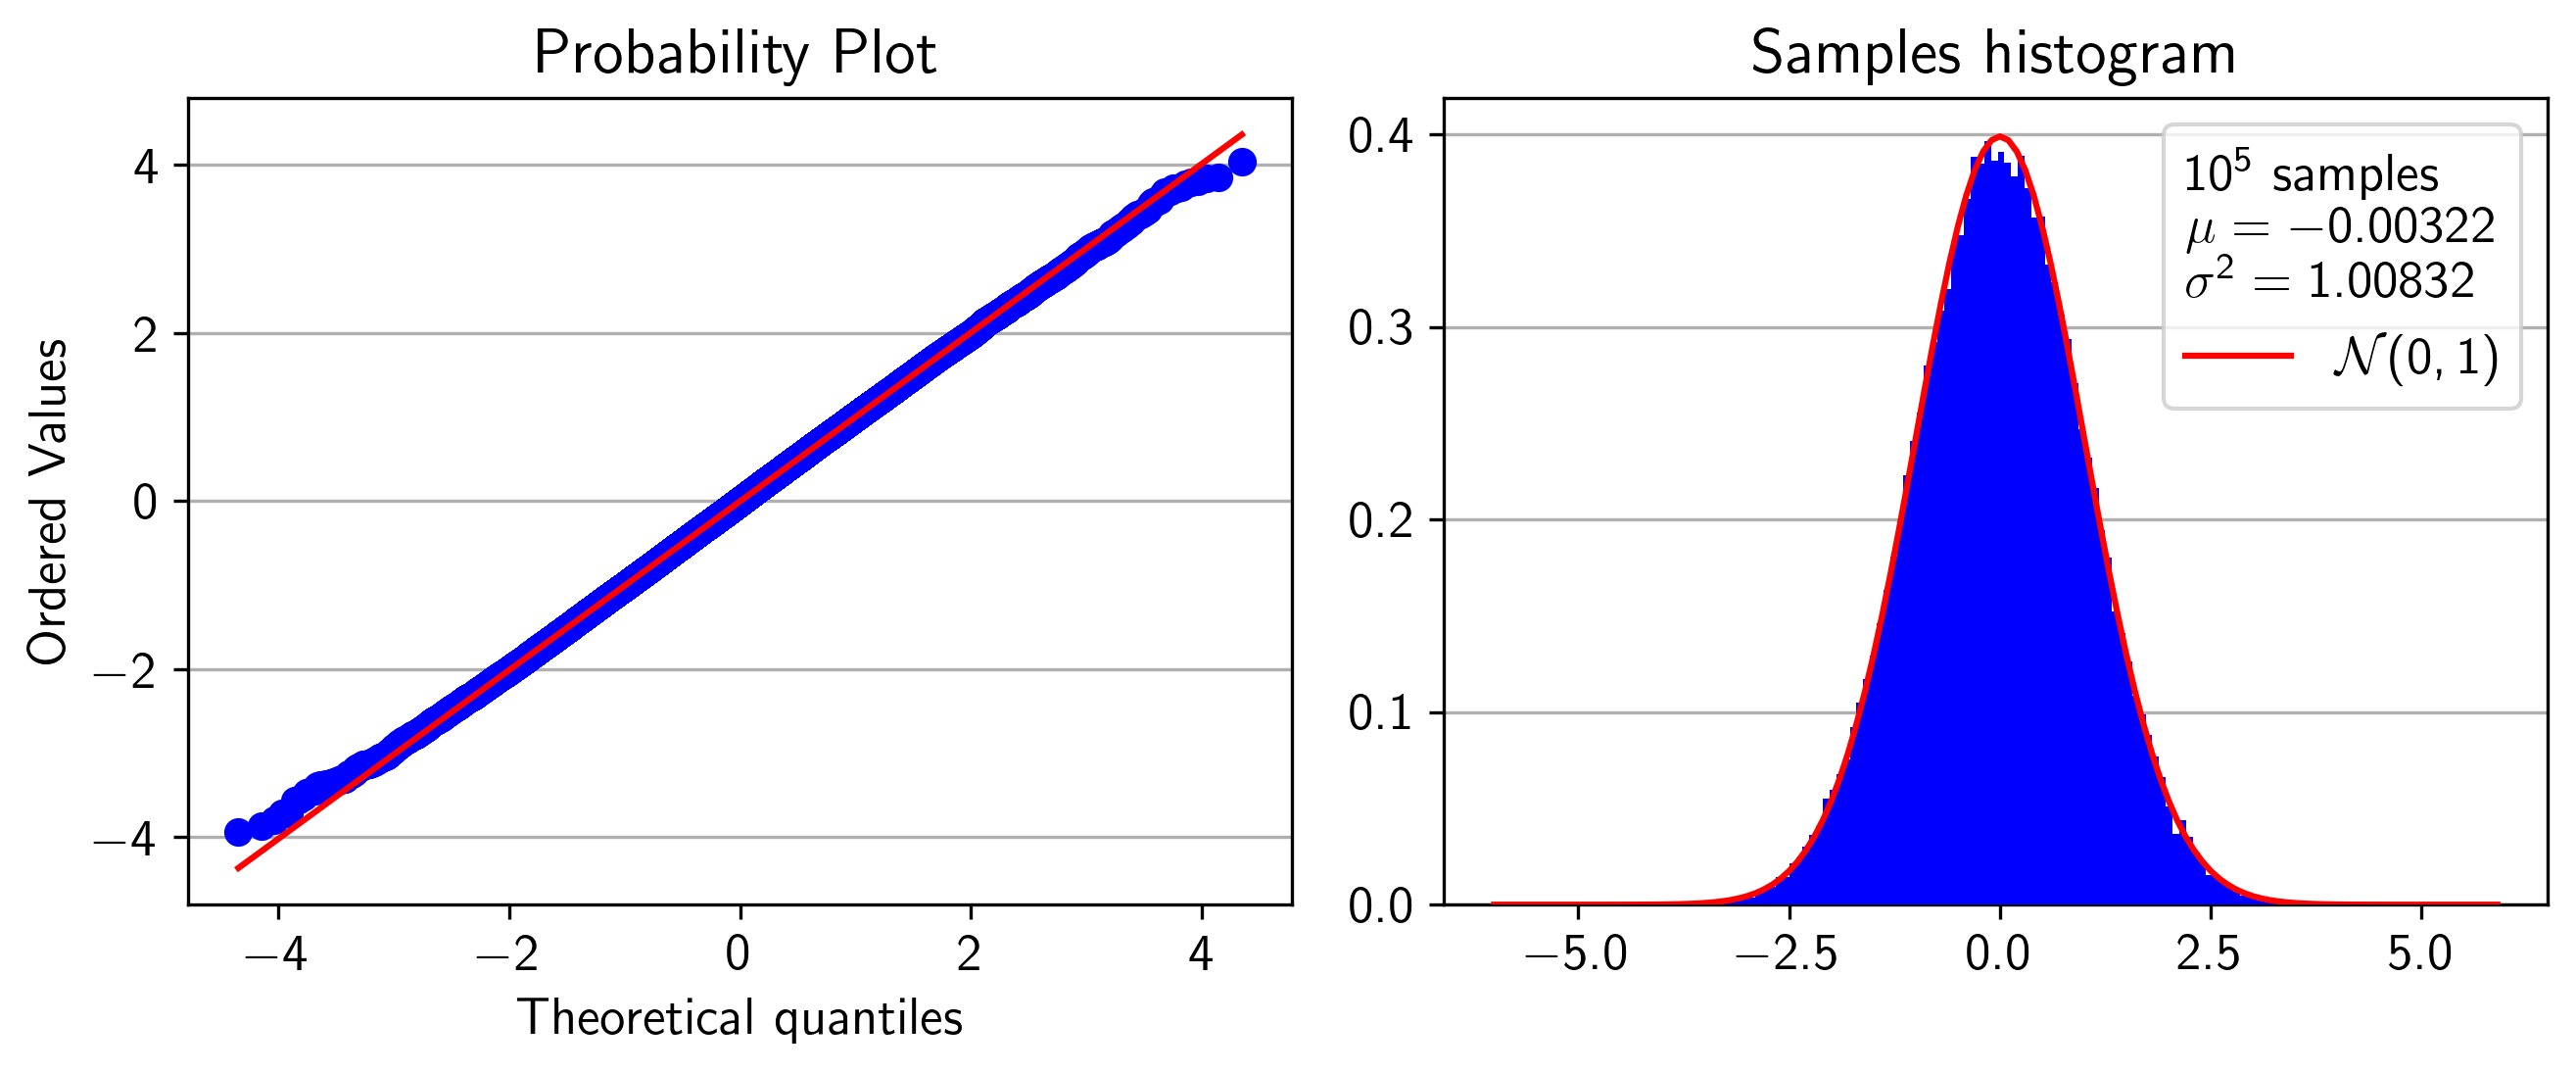
\includegraphics[width=\textwidth]{root/Imagenes/4_bnn_riscv/gaus_aprox.png}
    \caption{Análisis estadístico de $10^5$ muestras del GRNG implementado (azul) con respecto a $\mathcal{N}(0,1)$ (rojo). A la izquierda se muestra un gráfico Q-Q. A la derecha se muestra un histograma.}
    \label{fig:gauss_aprox}
\end{figure}

\subsubsection{Muestreo de una distribución uniforme}

Para generar muestras de distribuciones uniformes se utiliza una versión del algoritmo Xorshift de 32 bits \cite{xorshift}. Es un algoritmo sencillo para generar números pseudoaleatorios solamente con instrucciones \texttt{xor} y \texttt{shift}.

\subsection{Conversor de modelos}

Se ha desarrollado una herramienta en Python que convierte modelos BNN TensorFlow ya entrenados en precisión de punto flotante a ficheros de código C que puedan ejecutarse junto al motor de inferencia explicado en la Sección \ref{sec:motor_inferencia_c}. Esta herramienta realiza las siguientes tareas:

\begin{itemize}
    \item Transformar los pesos a coma fija.
    \item Analizar la precisión mínima necesaria. Buscar el tamaño de dato más pequeño en los que los pesos transformados se puedan almacenar. \todo
    \item Generar vectores de pesos. Generar código C que almacene los pesos en vectores aplanados.
    \item Generar función de inferencia. Analizar que capas forman el modelo y generar el código de una función de inferencia utilizando las funciones proveídas por el motor.
    \item Transformar los datos de prueba a coma fija.
    \item Generar vector de datos de prueba.
\end{itemize}

\subsection{Verificación automática}

Para analizar el correcto funcionamiento del motor de inferencia y estudiar el impacto en el rendimiento de las optimizaciones posteriores se ha desarrollado una herramienta que compara las predicciones del conjunto de datos de prueba obtenidas con el motor de inferencia y TensorFlow de forma automática. 

\subsubsection{Modelos}

Durante el proceso de verificación se han utilizado tres arquitecturas de modelos diferentes. La Tabla \ref{tab:hyper_models} muestra la arquitectura de los modelos para clasificación de píxeles hiperespectrales \cite{bnn_hyper_uncertainty}. Los conjuntos de datos utilizados para este modelo son diferentes imágenes hiperespectrales obtenidas mediante satélite denominadas BO, IP, KSC, PU y SV.

\begin{table}[h]
    \centering
    \caption{Arquitectura de los modelos para clasificación de píxeles hiperespectrales.}
    \label{tab:hyper_models}
    \begin{tabular}{lll}
    \hline
         \textbf{Layer Type} & \textbf{Input} & \textbf{Output}\\ \hline
         Dense & Number of spectral bands & 32\\
         Dense & 32 & 16\\
         Dense & 16 & Number of pixel classes\\ \hline
    \end{tabular}
\end{table}

La Tabla \ref{tab:cnn_models} muestra una arquitectura LeNet-5 bayesiana. LeNet-5 es una arquitectura de red neuronal convolucional (\textit{\textbf{C}onvolutional \textbf{N}eural \textbf{N}etwork}) simple \cite{lenet}. Se ha entrenado un modelo con la misma arquitectura para reconocer el conjunto de datos MNIST \cite{MNIST_dataset} y CIFAR-10 \cite{CIFAR_dataset} pero utilizando capas bayesianas.

\begin{table}[h]
    \centering
    \caption{Arquitectura LeNet-5 bayesiana.}
    \label{tab:cnn_models}
    \begin{tabular}{llll}
        \hline
         \textbf{Layer Type} &  \textbf{Input} &  \textbf{Output} & \textbf{Kernel Size} \\ \hline
         Conv2D Valid & 28$\times$28 & 24$\times$24$\times$6 & 5$\times$5 \\
         MaxPool2D & 24$\times$24$\times$6 & 12$\times$12$\times$6 & 2$\times$2 \\
         Conv2D Valid & 12$\times$12$\times$6 & 8$\times$8$\times$16 & 5$\times$5 \\
         MaxPool2D & 8$\times$8$\times$16 & 4$\times$4$\times$16 & 2$\times$2 \\
         Conv2D Valid & 4$\times$4$\times$16 & 1$\times$1$\times$120 & 4$\times$4 \\
         Dense & 120 & 84 & \\
         Dense & 84 & 10 & \\ \hline
    \end{tabular}
\end{table}

La Tabla \ref{tab:b2n2_model} muestra la arquitectura B2N2, propuesta por Awano \emph{et al.} junto a su acelerador para BNN \cite{bnn_clt_approx}. También se ha entrenado para reconocer los conjuntos de datos MNIST y CIFAR-10.

\begin{table}[h]
    \centering
    \caption{Arquitectura B2N2.}
    \label{tab:b2n2_model}
    \begin{tabular}{llll}
    \hline
    \textbf{Layer Type} & \textbf{Input} & \textbf{Output} & \textbf{Kernel Size}\\ \hline
    Conv2D Same & 32$\times$32 & 32$\times$32$\times$32 & 3$\times$3 \\
    Conv2D Same & 32$\times$32$\times$32 & 32$\times$32$\times$32 & 3$\times$3 \\
    MaxPool2D & 32$\times$32$\times$32 & 16$\times$16$\times$32 & 2$\times$2 \\
    Conv2D Same & 16$\times$16$\times$32 & 16$\times$16$\times$64 & 3$\times$3 \\
    Conv2D Same & 16$\times$16$\times$64 & 16$\times$16$\times$64 & 3$\times$3 \\
    MaxPool2D & 16$\times$16$\times$64 & 8$\times$8$\times$64 & 2$\times$2 \\
    Conv2D Same & 8$\times$8$\times$64 & 8$\times$8$\times$128 & 3$\times$3 \\
    Conv2D Same & 8$\times$8$\times$128 & 8$\times$8$\times$128 & 3$\times$3 \\
    MaxPool2D & 8$\times$8$\times$128 & 4$\times$4$\times$128 & 2$\times$2 \\
    Dense & 2028 & 10 & \\ \hline
    \end{tabular}
\end{table}

\subsubsection{Métricas}

Para comparar los conjuntos de predicciones se han utilizado las métricas de incertidumbre y la precisión. Analizar las métricas de incertidumbre y las propiedades estadísticas de los modelos es complejo. Para hacerlo se han utilizado 4 tipos de gráficas de las que se puede ver un ejemplo en la Figura \ref{fig:figure_example}. Estas gráficas se han creado utilizando las predicciones para el conjunto de datos de píxeles hiperespectrales KSC.

\ref{fig:example_hist} muestra un histograma de la incertidumbre agrupada por aciertos y fallos. \ref{fig:example_class} muestra la incertidumbre media, separada en epistémica y aleatoria, de las predicciones de cada clase. \ref{fig:example_acc_unc} muestra la precisión con respecto a la incertidumbre junto con un histograma de los datos agrupados también con respecto a la incertidumbre. \ref{fig:example_calibration} muestra la recta de calibración del modelo.

\begin{figure}[H] % Si no se usa H hace un accidente de tren
     \centering
     \begin{subfigure}[b]{0.48\textwidth}
         \centering
         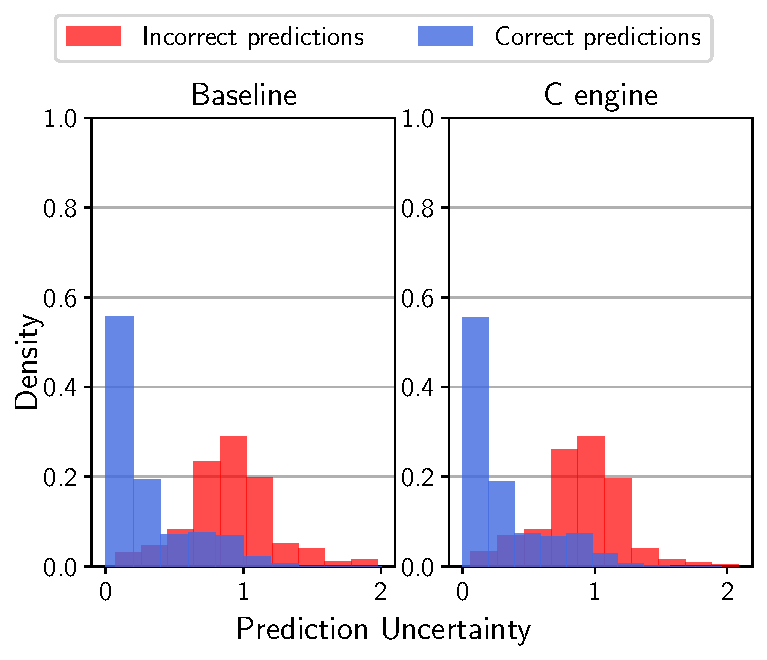
\includegraphics[width=\textwidth]{root/Imagenes/4_bnn_riscv/hist_predictions.pdf}
         \caption{Histogramas de incertidumbre divididos en predicciones correctas (azul) y predicciones incorrectas (rojo).}
         \label{fig:example_hist}
     \end{subfigure}
     \hfill
     \begin{subfigure}[b]{0.48\textwidth}
         \centering
         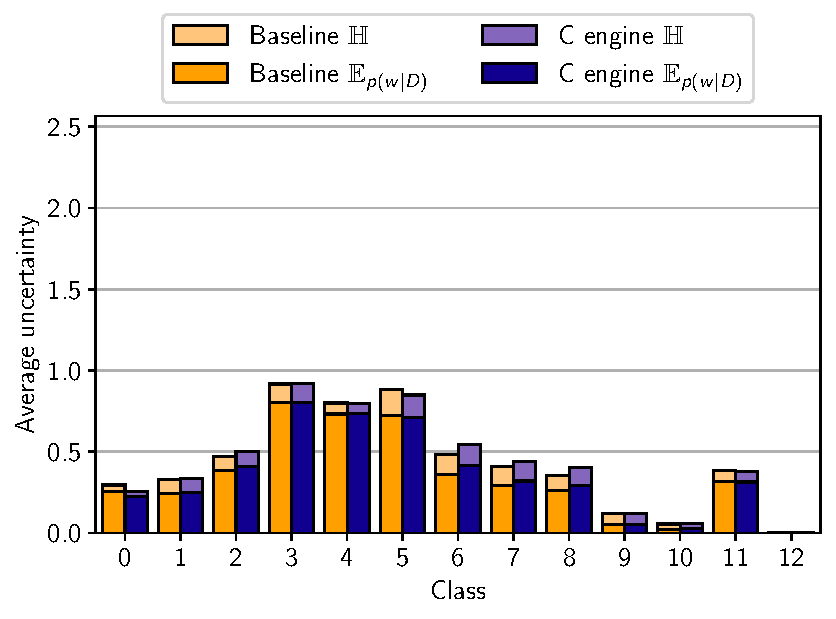
\includegraphics[width=\textwidth]{root/Imagenes/4_bnn_riscv/class_uncertainty.pdf}
         \caption{Incertidumbre predictiva ($\mathbb{H}$) y aleatoria ($\mathbb{E}p$) agrupada por clases.\\}
         \label{fig:example_class}
     \end{subfigure}
     \hfill
     \begin{subfigure}[b]{0.48\textwidth}
         \centering
         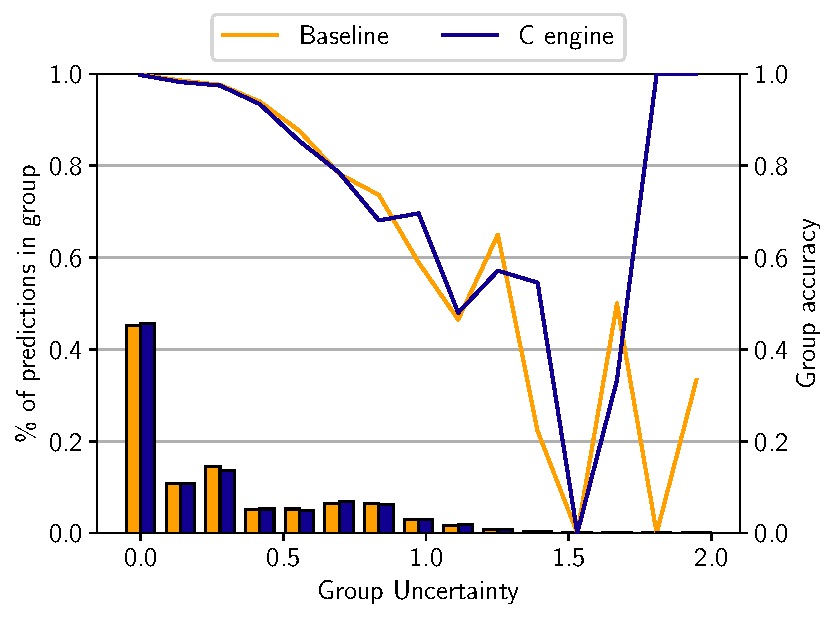
\includegraphics[width=\textwidth]{root/Imagenes/4_bnn_riscv/acc_vs_unc.pdf}
         \caption{Precisión y porcentaje de predicciones agrupadas por incertidumbre.\\}
         \label{fig:example_acc_unc}
     \end{subfigure}
     \hfill
     \begin{subfigure}[b]{0.48\textwidth}
         \centering
         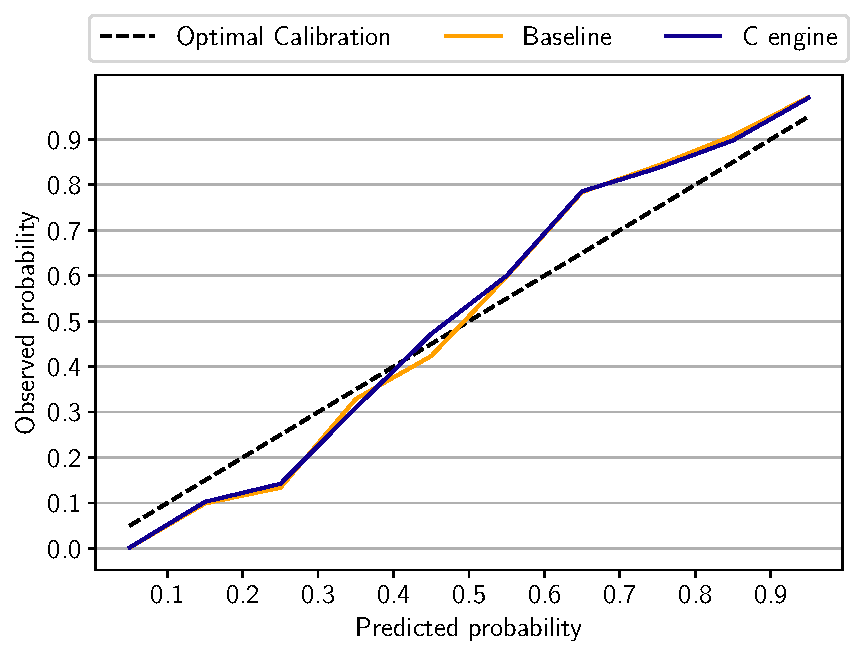
\includegraphics[width=\textwidth]{root/Imagenes/4_bnn_riscv/calibration.pdf}
         \caption{Recta de calibración del modelo, muestra probabilidades observadas con respecto a las probabilidades predichas por el modelo.}
         \label{fig:example_calibration}
     \end{subfigure}
        \caption{Ejemplos de gráficas para analizar la incertidumbre y propiedades estadísticas de un modelo BNN. En \ref{fig:example_class}, \ref{fig:example_acc_unc} y \ref{fig:example_calibration} los colores amarillos representan los resultados obtenidos con TensorFlow y los colores azules los obtenidos con el motor de inferencia desarrollado. Predicciones del conjunto de prueba de píxeles hiperespectrales KSC.}
        \label{fig:figure_example}
\end{figure}

Como se muestra en el ejemplo se obtienen resultados muy similares en todas las gráficas. Las únicas diferencias notables se aprecian en las rectas de precisión de la Figura \ref{fig:example_acc_unc}, pero estas diferencias ocurren en predicciones con incertidumbre alta de las que además hay muy pocas. El modelo al reportar una incertidumbre elevada ya esta avisando de la baja fiabilidad de la predicción con lo que diferencias en este tipo de predicciones son esperables y aceptables. Para el resto de modelos se obtienen resultados con las mismas similitudes entre motores de inferencia, se pueden consultar todos en el Anexo \ref{}.

La precisión es el ratio de predicciones correctas sobre el número total de predicciones. la Tabla \ref{tab:engine_acc} muestra la precisión obtenida con los diferentes modelos utilizando ambos motores de inferencia. Al tratarse de modelos probabilísticos pequeñas fluctuaciones son esperables, especialmente en las predicciones con mucha incertidumbre.

\begin{table}[ht]
\centering
\caption{Comparación de precisión obtenida con el motor de inferencia implementado con respecto a resultados obtenidos con TensorFlow}
\label{tab:engine_acc}
\begin{tabular}{lll}
\hline
 &  \multicolumn{2}{c}{\textbf{Motor de inferencia}}\\
 \textbf{Modelo} & \textit{TensorFlow} & \textit{C} \\ \hline
 Hiperespectral BO   & 0.9039 & 0.9101 \\
 Hiperespectral IP   & 0.8139 & 0.8148 \\
 Hiperespectral KSC  & 0.9256 & 0.9217 \\
 Hiperespectral PU   & 0.9017 & 0.9021 \\
 Hiperespectral SV   & 0.9257 & 0.9275 \\
 Lenet-5 MNIST      & 0.9836 & 0.9830 \\
 Lenet-5 CIFAR10    & 0.6351 & 0.6229 \\
 B2N2 MNIST         & 0.9872 & 0.9854 \\
 B2N2 CIFAR10       & 0.7295 & 0.7134 \\\hline
\end{tabular}
\end{table}

Los resultados demuestran que el motor de inferencia desarrollado incluso tras transformar los datos a coma fija y perder precisión en la representación no perjudica a las métricas de incertidumbre ni a la precisión.

\section{Análisis de la carga de trabajo}

La principal operación en la inferencia de NN es \textit{\textbf{M}ultiply–\textbf{AC}cumulate} (MAC), mostrada en la Ecuación \ref{eq:mac}. Una capa es un conjunto de neuronas, las entradas a una neurona $x_i$ se multiplican por sus pesos $w_i$ y se acumulan junto a al \textit{bias} $b$. Una capa no convolucional se puede representar como una única multiplicación de matriz vector.
\begin{equation} \label{eq:mac}
b + \sum_{i=0}^N w_i x_i
\end{equation}

En el caso de las BNN estas operaciones MAC además requieren muestrear una distribución gaussiana, como se muestra en la Ecuación \ref{eq:bnn_mac}.
\begin{equation} \label{eq:bnn_mac}
b + \sum_{i=0}^N Sample(\mu_i, \sigma_i)\ x_i
\end{equation}

El procesador RISC-V tiene un contador de ciclos disponible llamado \texttt{mcycle}, lo que permite medir prestaciones con precisión a nivel de ciclo. Se ha utilizado este contador para crear un perfil de la carga de trabajo del motor de inferencia, el cual se muestra en la Figura \ref{fig:cycle_profile}.

\begin{figure}[h]
    \centering
    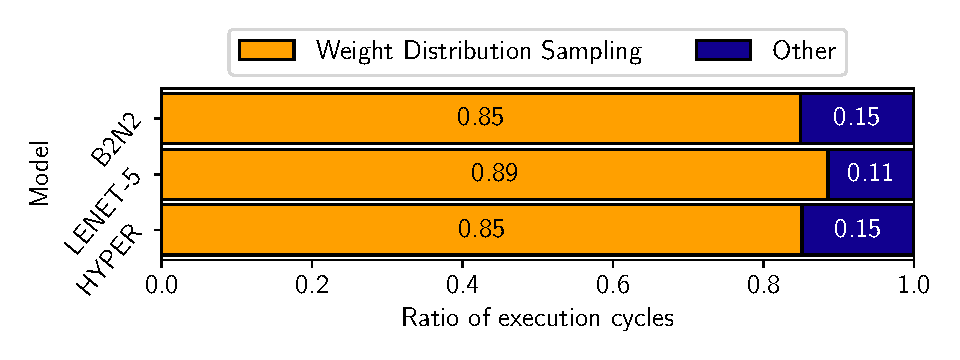
\includegraphics[width=0.9\textwidth]{root/Imagenes/4_bnn_riscv/cycles.pdf}
    \caption{.}
    \label{fig:cycle_profile}
\end{figure}

La operación de muestreo de la distribución es la más costosa con diferencia, ocupando mas del 80\% de los ciclos en los 3 modelos diferentes. Por ello, uno de los objetivos principales de este trabajo y de otros relacionados ha sido optimizar esta operación.

\section{Optimizaciones software}

Awano \emph{et al.} propusieron muestrear distribuciones Bernoulli obteniendo el parámetro de las mismas mediante una transformación de los parámetros de las distribuciones gaussianas \cite{bnn_clt_approx}. Se intentó replicar este método mediante software pero los resultados obtenidos no fueron los esperados.

Este trabajo propone un método basado en el suyo pero utilizando distribuciones Uniformes en vez de distribuciones Bernoulli. Como las BNN integran modelado probabilístico hay que tener en cuenta las esperanzas y varianzas de las operaciones MAC, estas se muestran en las Ecuaciones \ref{eq:neuron_expected} y \ref{eq:neuron_variance}
\begin{equation} \label{eq:neuron_expected}
E\left[ b + \sum_{i=0}^N w_i x_i \right]  = b + \sum_{i=0}^N ( E[w_i] E[x_i] )
\end{equation}
\begin{equation} \label{eq:neuron_variance}
V\left[ b + \sum_{i=0}^N w_i x_i \right] = \sum_{i=0}^N ( V[w_i]V[x_i] + V[w_i]E[x_i]^2 + V[x_i]E[w_i]^2 )
\end{equation}

Considerando un peso $w \sim \mathcal{N}(\mu,\sigma)$, se define uno nuevo $w' = b u + a$, siendo $u$ una muestra de una distribución unifome $\mathcal{U}(0,1)$. 

Para calcular $a$ y $b$ se resuelve el sistema de ecuaciones $\mu = E[w']$, $\sigma^2 = V[w']$

\begin{equation} \label{eq:neuron_variance}
\mu = \dfrac{b}{2} + a
\end{equation}
\begin{equation} \label{eq:neuron_variance}
\sigma^2 = \dfrac{b^2}{12}
\end{equation}
\begin{equation} \label{eq:system_a}
a = \mu - \dfrac{b}{2}
\end{equation}
\begin{equation} \label{eq:system_b}
b = \sigma \sqrt{12}
\end{equation}
